
\documentclass{beamer}
\beamertemplatenavigationsymbolsempty
\usepackage{amsmath, amssymb, hyperref, graphics, tikz}
%\usepackage{mathpazo, soul}



\newcommand{\C}{\mathbb{C}}
\newcommand{\Z}{\mathbb{Z}}
\newcommand{\R}{\mathbb{R}}
\newcommand{\N}{\mathbb{N}}
\DeclareMathOperator{\Real}{Re}
\DeclareMathOperator{\Imag}{Im}


\begin{document}


\begin{frame}{Today: Consequences of the Cauchy-Riemann Equations}

We ended last time by proving:  
\begin{theorem}[Cauchy-Riemann Equations]
  For $z=x+iy$, write $f(z)=u(x,y)+iv(x,y)$ with $u,v$ real.  Then if $f$ is differentiable at $z_0$, we have:
  $$\frac{\partial u}{\partial x}=\frac{\partial v}{\partial y}\quad\quad\frac{\partial u}{\partial y}=-\frac{\partial v}{\partial x}\quad \text{ at } z_0$$
\end{theorem}

\begin{block}{Today: what does this tell us about $f$?}
  \begin{enumerate}
  \item Silly, but easy to examine: If $u,v$ are related in any other way, $f$ is \emph{highly} constrained
  \item Important, but not traditionally examined: $f$ is a \emph{conformal mapping}
  \item Important, examined: The real and imaginary parts of $f$ are \emph{harmonic}
  \end{enumerate}   


  \end{block}

\end{frame}

\begin{frame}{Section 5.8: When $u$ and $v$ are related}

\begin{itemize}
    \item Cauchy-Riemann relates between $\Real(f)$ and $\Imag(f)$
    \item If we have more relations, then $f$ is \emph{very} constrained
\end{itemize}


\begin{example}[Similar to those in notes]
Suppose that $f$ is differentiable on a connected domain, and that its real and imaginary parts satisfy $u=v^2$.  Prove that $f$ is constant.

  \end{example}

\end{frame}

\begin{frame}{Holomorphic functions are conformal maps}

  In MAS211 you looked at the derivative of a map $f:\R^n\to\R^m$ as a linear map $Df:\R^n\to\R^m$, and hence as a matrix.  The entries are the partial derivatives, so for $f:\C\to\C$

  $$Df=\begin{bmatrix}\frac{\partial u}{\partial x} & \frac{\partial u}{\partial y} \\ \frac{\partial v}{\partial x} & \frac{\partial v}{\partial y} \end{bmatrix}$$

  If $f:\C\to\C$ is differentiable at $z_0$, this linear map corresponds to multiplication by the complex number $f^\prime(z_0)=a+bi$. The Cauchy-Riemann equations just enforce this: 

$$Df(z_0)=\begin{bmatrix} a & -b \\ b & a \end{bmatrix}=r\begin{bmatrix} \cos(\theta) & -\sin(\theta) \\ \sin(\theta) & \cos(\theta)\end{bmatrix}$$

Hence the derivative is a rotation + a scaling, and \emph{preserves angles}. Such a map from $\R^2\to\R^2$ is called \emph{conformal}.


    \end{frame}

\begin{frame}{Motivation for harmonic functions: important PDEs}
The Laplacian operator, written $\nabla^2$ or $\Delta$, acts on functions $g:\R^2\to\R$ by
$$\nabla^2g=\nabla\cdot\nabla g=\frac{\partial^2 g}{\partial x^2}+\frac{\partial^2 g}{\partial y^2}$$
and occurs in many PDEs important in applied math.  

\begin{block}{Examples}
Let $f(x,y,t)$ be a function of two space variables and one time variable.
\begin{itemize}
    \item The heat equation $\frac{\partial f}{\partial t}=\nabla^2f$
    \item The wave equation $\frac{\partial^2 f}{\partial t^2}=\nabla^2f$
\end{itemize}
\end{block}
A steady state solution to either of these equations would be $\nabla^2f=0$.  
\end{frame}

\begin{frame}{Harmonic Functions}
\begin{definition}
A function $u:\R^2\to\R$ is \emph{harmonic} if $\nabla^2f=0$
\end{definition}

\begin{lemma}Let $f(z)=u(x,y)+iv(x,y)$ be analytic on a domain $D$.  Then $u$ and $v$ are harmonic on $D$
\end{lemma}
\begin{proof} Cauchy-Riemann equations + mixed partials are equal.
\end{proof}
This gives us lots of harmonic functions.  
\begin{block}{Does this give us \emph{all} harmonic functions?}
Given a harmonic function $u(x,y)$ on a domain, is it the real part of an analytic function $f(z)$?
\end{block}
Yes, on a \emph{simply-connected} domain.

\end{frame}

\begin{frame}{When is $u$ are the real part of analytic functions?}
\begin{block}{From the 2012-2013 exam}
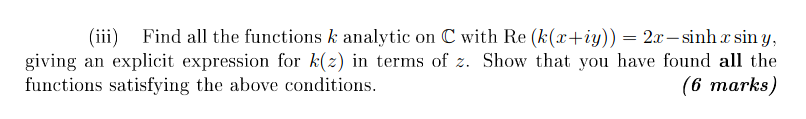
\includegraphics[width=\textwidth,height=0.8\textheight,keepaspectratio]{RealPart2012.png}
\end{block}

\begin{block}{The real part of an analytic function is harmonic}
First, check $\nabla^2u=0$.  If not, the answer is no.
\end{block}

\begin{block}{If it is, find $f^\prime$ using Cauchy-Riemann}
$$f^\prime=\frac{\partial}{\partial x} \Big(u(x,y)+iv(x,y)\Big)=u_x+iv_x=u_x-iu_y$$
\end{block}

This gives us $f^\prime$ in terms of $x$ and $y$.  We'd \emph{like} to write $f^\prime$ in terms of $z$, and integrate to find $f$. But how?

\begin{block}{Maybe we need a clever little trick....}
\end{block}

\end{frame}

\begin{frame}{Dr. Hart's "Clever little trick"}
\begin{block}{Given:}
We know $f^\prime$ in terms of $x$ and $y$, want it terms of $z$.
\end{block}

\begin{block}{Guess:}
Set $y=0$; to get $f^\prime(x)$ in terms of just $x$.  Integrate to get $f(x)$.  Guess that this is actually formula for $f(z)$
\end{block}

\begin{block}{Check:}
Show that $\Real(f)=u(x,y)$
\end{block}
\begin{block}{To find \emph{all} such $k$:}
\begin{lemma}Suppose that $f$ and $g$ are analytic on a region $D$ and that $\Real(f)=\Real(g)$ on $D$.  Then $f=g+ia$ for some $a\in\R.$
\end{lemma}
\end{block}

\end{frame}




\end{document}
